\documentclass[artMGITG,SIG,accept,moreauthors,font4]{mgitg}%,pdftex

%=====================================================
\usepackage{multirow}
\usepackage{subfigure}
\usepackage{longtable}
% \usepackage{graphicx}


%-- Interlineado ----------------------
% \renewcommand{\baselinestretch}{1.5}
%--------------------------------------

\makeatletter 

\makeatother
\articlenumber{2}
\pubvolume{1}
\issuenum{1}
\pubyear{2020}
\isbnnum{2711-3558 (En línea)}
\copyrightyear{2020}

%-- TITULO DEL ARTICULO -----------------------
\Title{Titulo del articulo ---Extenso---}
%----------------------------------------------

%-- AUTORES -----------------------------------
\Author{%
    Autor Uno$^{1}$*,
    Segundo Autor$^{2}$
    y
    Tercer Autor$^{3}$
    }
%----------------------------------------------

%-- AUTORES PARA LOS METADATOS DEL PDF --------
\AuthorNames{Autor Uno, Segundo Autor, Tercer Autor}
%----------------------------------------------

%-- AFILIACIÓN---------------------------------
\address{%
    $^{1}$ \quad Universidad Sergio Arboleda; Instituto Geográfico Agustín Codazzi-IGAC; autor.uno@usa.edu.co\\
    $^{2}$ \quad Universidad Sergio Arboleda; Instituto Geográfico Agustín Codazzi-IGAC; segundo@usa.edu.co\\
    $^{3}$ \quad Universidad Sergio Arboleda; Instituto Geográfico Agustín Codazzi-IGAC; segundo@usa.edu.co\\}
%----------------------------------------------

%-- INFORMACIÓN DE CONTACTO PARA AUTOR --------
\corres{Correspondencia: autor.uno@usa.edu.co}
%----------------------------------------------

%-- RESUMEN EN INGLÉS -------------------------
% Abstract (Do not insert blank lines, i.e. \\) 
% \abstract{{\color{red} Hace falta el abstract}}
%----------------------------------------------
%-- PALABRAS CLAVE EN INGLÉS ------------------
% \keyword{{\color{red} y las keywords}}
%----------------------------------------------

%-- RESUMEN EN ESPAÑOL ------------------------
% Abstract (Do not insert blank lines, i.e. \\) 
\resumen{Texto para el resumen.}
%----------------------------------------------
%-- PALABRAS CLAVE EN ESPAÑOL -----------------
\palabrasclave{kw1, kw2, kw3, kw4.}
%----------------------------------------------

\setcounter{secnumdepth}{4}


%-- Aquí empieza el documento -------------------
\begin{document}
%
%-- INTRODUCCIÓN -----------------
\section{Introducción}
%
\noindent
Lorem ipsum dolor sit amet, consectetur adipiscing elit. Nullam sodales, purus a varius sollicitudin, nibh magna mattis erat, nec sodales est sapien nec purus. Vivamus a varius turpis, sed feugiat orci. Morbi et laoreet lacus. Praesent feugiat massa quis metus blandit tempus. Donec in ornare erat. Morbi ut lectus vel ante fermentum pharetra. Vivamus ut nisi mi. Aenean rhoncus ut nisl vitae maximus. Etiam id fermentum dui. Duis eu orci non libero egestas bibendum. Curabitur quis mi sem. Donec at gravida augue. Donec quis iaculis sem. Nulla efficitur odio nisi, imperdiet fermentum lectus ullamcorper at. Praesent leo mi, ultricies et sapien eu, vestibulum sagittis sem \cite{Ref01,Ref12,Ref13}.

Sed quis risus ac mi bibendum egestas ac et nisi. Donec nec elit lorem. Integer arcu ipsum, interdum sed ipsum eget, molestie blandit sem. Ut lacus erat, auctor nec consequat ut, sagittis a neque. Phasellus volutpat tortor et turpis viverra accumsan. Sed condimentum tellus eget erat euismod tristique. Sed eu ante felis. Quisque est nisl, bibendum sodales felis sit amet, laoreet lobortis lacus. Suspendisse pretium dictum diam vel molestie. Vivamus bibendum elementum rhoncus. Nullam pretium nunc vel massa pretium tristique (ver Figura \ref{fig1}). 

\begin{figure}[!ht]
    \centering
    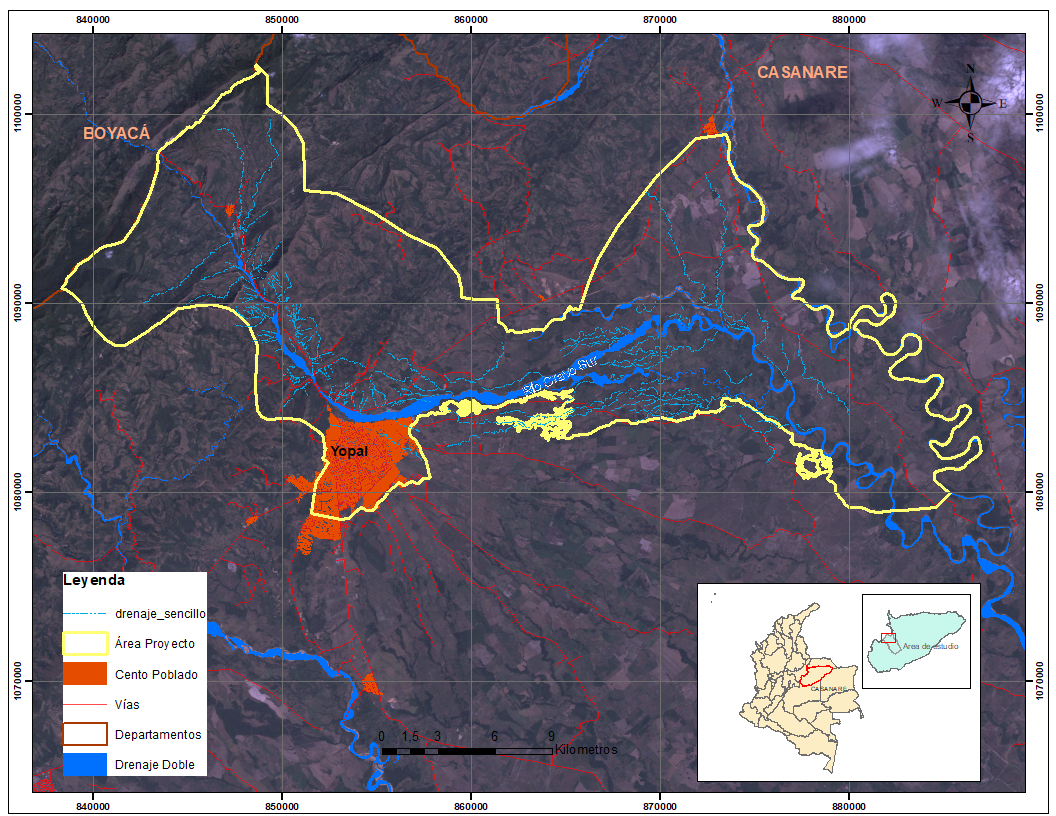
\includegraphics[width=0.8\textwidth]{figuras/figura1}
    \caption{Espectro de reflectancia de algunos materiales de la superficie de la tierra: agua, vegetación, suelos y rocas}
    \label{fig1}
\end{figure}


\begin{figure}[!ht]
    \centering
    \subfigure[Porcentaje de las iniciativas desarrolladas por diferentes países a nivel internacional]
        {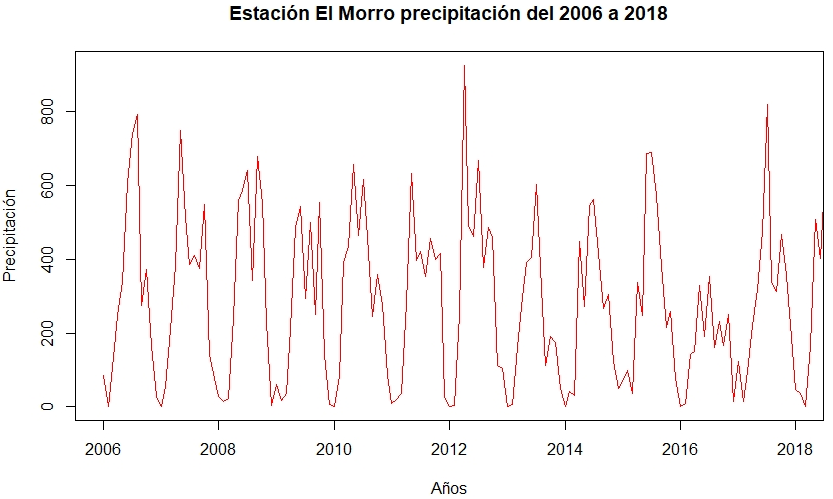
\includegraphics[width=0.4\textwidth]{figuras/figura4a}\label{fig3a}}
    \hfill
    %
    \subfigure[Porcentaje según el tipo de iniciativa: desarrollo software, estándares, entre otros]
        {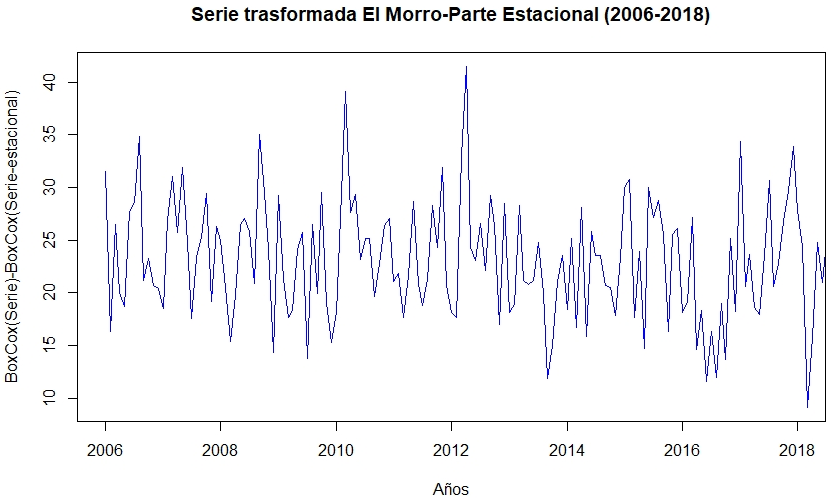
\includegraphics[width=0.475\textwidth]{figuras/figura4b}\label{fig3b}}
    \caption{Iniciativas a nivel mundial}
    \label{fig3}
\end{figure}


%-- MATERIALES Y MÉTODOS ------------------------
\section{Materiales y métodos}
%
\noindent
Proin tempor vitae nibh et efficitur. Done c commodo ultricies magna, id pretium justo malesuada ut. Aenean tristique ultricies rutrum. Phasellus egestas nec odio quis ullamcorper. Mauris a est eu leo malesuada maximus ac eu lacus. Nullam scelerisque placerat risus, non malesuada arcu iaculis in. Quisque quis lacus vulputate, semper tellus at, efficitur elit. Sed et pellentesque mi.

%-- RESULTADOS ------------------------
\section{Resultados}
%
\unskip
\subsection{Desarrollo del modelo ARIMA} 
%
\noindent
Praesent volutpat ante eu aliquet finibus. Etiam id hendrerit nibh. Aliquam ut pellentesque elit. Nam in dolor eget velit pharetra dapibus ut sollicitudin augue. Morbi lacinia quam sem, sit amet consequat nibh molestie ac. Ut at mi quis nisl venenatis lacinia. Donec suscipit turpis et varius porttitor. Maecenas sed eleifend enim, vitae dapibus nisi.

Integer tincidunt fringilla lacus, at tincidunt lectus vulputate at. Phasellus vel rhoncus elit, eget pulvinar mi. Mauris quis porttitor diam. Suspendisse non eleifend ex, a aliquet mauris. Nulla facilisi. Nullam a nisi in leo iaculis pretium. Proin dolor nibh, pharetra in neque at, tempor dictum ante. Aenean id convallis metus. Etiam aliquam molestie lorem a laoreet. Sed lorem odio, ultrices id semper at, egestas suscipit magna. Suspendisse facilisis eu velit facilisis feugiat. Etiam porttitor, diam eu condimentum finibus, magna lacus elementum enim, non tempus diam diam sed leo (ver Tabla \ref{tab1}). 

\begin{table}[!ht]
    
    \centering
        \caption{Grupos de información incluidos en el metadato de la firma espectral en el SIEC y su número de atributos}
    % \begin{tabular}{p{0.3\textwidth}p{0.175\textwidth}p{0.35\textwidth}}
    % \resizebox{.95\textwidth}{!}{\begin{minipage}{\textwidth}
    \begin{tabular}{lll}
    \toprule
    Atributos del conjunto de datos & Atributos del sensor & Atributos del dato de la firma espectral\\
    \midrule
    Identificación (23)  & Instrumento (3) & Información del dato (14)\\[10pt]
    %
    Información de identificación del & Características del & Propiedades genéricas del dato (1)\\
    recurso (38) & instrumento (18) & \\[10pt]
    %
    Información de linaje (3)	& Iluminación (6) & Geometría del dato o firma (5)\\[10pt]
    %
    Información del sistema de & Instrumentación (accesorios  & Condiciones ambientales en el\\
    referencia (3)  & de campo)~(6) &  momento de la toma (7)\\[10pt]
    %
    Información de distribución (4)	& & \\
    \bottomrule
    \end{tabular}
    \label{tab1}
    % \end{minipage} }
\end{table}




%%%%%%%%%%%%%%%%%%%%%%%%%%%%%%%%%%%%%%%%%%
\section{Discusión}
%
\noindent
Maecenas facilisis diam vitae libero volutpat, vel convallis ligula posuere. Maecenas finibus pharetra consequat. Ut cursus nibh pellentesque nisl faucibus, vel maximus massa laoreet. In sed auctor enim. Etiam mi velit, porta non scelerisque sit amet, pharetra at ante. Proin porttitor diam ipsum, varius facilisis ligula vestibulum in. Duis id nunc varius, hendrerit quam sit amet, dictum tellus.

Donec pretium, dolor non sagittis vehicula, sapien turpis congue turpis, ac ultricies turpis nibh id velit. Nullam quis vehicula mi, ut bibendum erat. Suspendisse sed quam eget lacus ornare mollis. Sed consequat bibendum augue id congue. Phasellus luctus odio sit amet sapien lacinia semper. Suspendisse feugiat, orci eu faucibus dignissim, tellus tortor laoreet purus, vel luctus arcu sapien nec nisl. Praesent rhoncus finibus purus, a suscipit dolor vestibulum vel. Curabitur laoreet bibendum accumsan. Suspendisse potenti. Maecenas placerat mollis purus, tincidunt sodales sapien. 


\section{Conclusiones}
%
\noindent
Etiam et lacus vel sapien pretium interdum. Pellentesque pellentesque ultricies purus sed bibendum. Vestibulum finibus lorem a erat congue placerat id ut sem. Lorem ipsum dolor sit amet, consectetur adipiscing elit. Quisque ipsum velit, efficitur id commodo ut, fermentum vitae purus. Curabitur at elit placerat, dictum nibh eget, varius velit. Donec ut mauris et dolor porttitor posuere. Suspendisse ut vehicula purus. Donec cursus quam ornare mi egestas varius. Sed molestie sem vel euismod porttitor. Ut rhoncus fringilla interdum. Aliquam ultrices at ex eget auctor. Integer vel felis urna. 



%%%%%%%%%%%%%%%%%%%%%%%%%%%%%%%%%%%%%%%%%%
%\section{Patents}
%This section is not mandatory, but may be added if there are patents resulting from the work reported in this manuscript.

 
%%%%%%%%%%%%%%%%%%%%%%%%%%%%%%%%%%%%%%%%%%
\vspace{10pt} 

%%%%%%%%%%%%%%%%%%%%%%%%%%%%%%%%%%%%%%%%%%
% \acknowledgments{}

% Apendices
%\appendixtitles{no} 
%\appendix
%\section{}
%\input{tablasapendice.tex}






%%%%%%%%%%%%%%%%%%%%%%%%%%%%%%%%%%%%%%%%%%
\reftitle{Referencias}
% Please provide either the correct journal abbreviation (e.g. according to the “List of Title Word Abbreviations” http://www.issn.org/services/online-services/access-to-the-ltwa/) or the full name of the journal.
% Citations and References in Supplementary files are permitted provided that they also appear in the reference list here. 

%=====================================
% References, variant A: external bibliography
%=====================================
%\externalbibliography{yes}
\bibliography{referencias}

%=====================================
% References, variant B: internal bibliography
%=====================================
% \begin{thebibliography}{999}
%     \input{referencias.tex}
% \end{thebibliography}

\end{document}


% \begin{table}[!ht]
%     \centering
%         \caption{Imágenes multiespectrales procesadas}
%     \begin{tabular}{ccc}
%     \toprule
%     Sensor & Imagen & año\\
%     \midrule
%     ETM & LE07\_L1TP\_007056\_20070131\_20170105\_01\_T1 & 31/01/2007\\
%     ETM	& LE07\_L1TP\_007056\_20070216\_20170104\_01\_T1 & 16/02/2007\\
%     TM	& LT05\_L1TP\_007056\_20091214\_20161017\_01\_T1 & 14/12/2009\\
%     OLI	& LC08\_L1TP\_007056\_20140110\_20170426\_01\_T1 & 10/01/2014\\
%     OLI	& LC08\_L1TP\_007056\_20180206\_20180221\_01\_T1 & 21/02/2018\\
%     \bottomrule
%     \end{tabular}
%     \label{tab1}
% \end{table}